%!TEX root = ../figures.tex

\documentclass[tikz]{standalone}


\usepackage{tikz}
\usetikzlibrary{positioning,calc,fit,decorations.pathreplacing,arrows,positioning,backgrounds}
\renewcommand{\familydefault}{\sfdefault}

\usepackage{graphicx}
\usepackage{pxfonts}
\usepackage[T1]{fontenc}


%\definecolor{hivc}{cmyk}{0,0.80,0.83,0.13}                %\definecolor{hivc}{HTML}{DE2D26}
\definecolor{hivc}{RGB}{24,116,205}
\definecolor{selfc}{cmyk}{0,0,0,0.6}                      %\colorlet{selfc}{gray!80!white}


\begin{document}
\Huge


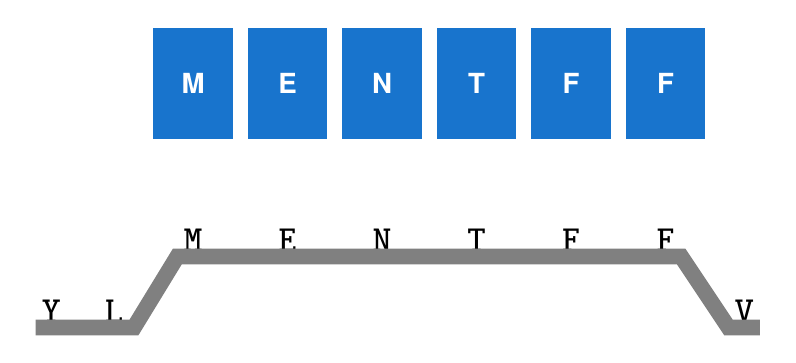
\begin{tikzpicture}
\colorlet{bgcol}{gray!15!white}
\tikzstyle{tcr}=[anchor=center,text=white,font=\bfseries];
\tikzstyle{eps}=[scale=1.3,anchor=south,text=black,font=\ttfamily];


\begin{scope}
      \foreach \x in {3.2,4.4,5.6,6.8,2,8}
        \filldraw[hivc] (\x,-0.7) rectangle +(1,1.4);

        \node[tcr] (t1) at (2.5,0) {M};
        \node[tcr] (t2) at (3.7,0) {E};
        \node[tcr] (t3) at (4.9,0) {N};
        \node[tcr] (t4) at (6.1,0) {T};
        \node[tcr] (t5) at (7.3,0) {F};
        \node[tcr] (t6) at (8.5,0) {F};
     
        \node[eps] at (0.7,-3.2) {Y};   
        \node[eps] at (1.5,-3.2) {L};
        \node[eps] at (2.5,-2.3) {M};
        \node[eps] at (3.7,-2.3) {E};
        \node[eps] at (4.9,-2.3) {N};
        \node[eps] at (6.1,-2.3) {T};
        \node[eps] at (7.3,-2.3) {F};
        \node[eps] at (8.5,-2.3) {F};
        \node[eps] at (9.5,-3.2) {V};
        
        \draw[gray,line width=2mm] (0.5,-3.1) -- (1.75,-3.1) -- (2.3,-2.2) -- (8.7,-2.2) -- (9.3,-3.1) -- (9.7,-3.1);
        
        
        %\node [fit=(A) (B) (C)] (fit) {};              

        
\end{scope}


\end{tikzpicture}

\end{document}


